% Contains all the older results etc. 
\subsection{Experimental evaluation}

Mainly centered around these evaluation questions:

\begin{enumerate}
\item What is the effect on the latency of high and low priority functions under various static cluster partitions?
\item What happens to cluster throughput?
\item Can cluster size be reduced? 
\item How does the dynamic partitioning affect performance under dynamic workloads? 
\end{enumerate}




\paragraph{Fixed cluster size.}
The high priority pool gets more servers. 

\begin{figure}
  \centering  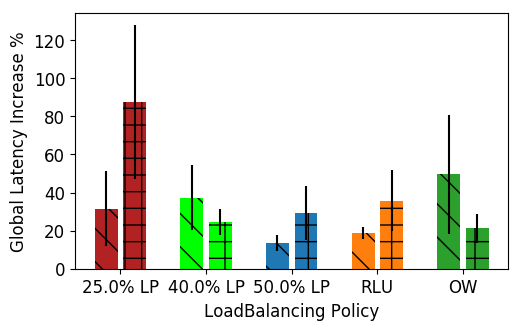
\includegraphics[width=0.4\textwidth]{../Figures/fixed/openload-latencies-cntnorm.png}
  \caption{Latencies with a fixed cluster size. Diagonal=High Priority.}
  \label{fig:fixed-lat}
\end{figure}


In this set of experiments, we are interested in examining the latency and throughput of the high and low priority pool.
Figure~\ref{fig:fixed-lat} shows the increase in function latency compared to their best-case warm start performance under no system load. The figure shows this latency increase, weighted by the relative frequency of the functions, to account for different function popularities. That is, we show sum of latency increase * function fraction in the workload.

For these series of experiments, we randomly and evenly divide the workload into high and low priority.
That is, half the function invocations are low priority, and the remaining half are high priority.
The ``OW'' and ``RLU'' categories in Figure~\ref{fig:fixed-lat} show the baseline performance in a single unpartitioned cluster.
50\% LP means that we assign half the cluster for low-priority functions, and we can see that this partitioning reduces the latency of high-priority functions by 10\% compared to RLU and by more than 3x compared to OpenWhisk.
This is a result of better locality and hence lower cold-starts and interference that we obtain through partitioning.

As we shrink the low-priority pool to only 25\% of the servers, the low-priority latency increases by 4x.

\textbf{Why are the high priority latencies changing and getting worse with bigger partitions? Locality? Stochastic load?}
\todocristina{About the comment above, I think it is locality (should be able to check this); BUT, the load balancing policy should help with this... why isn't it?}

\todocristina{In the figures, the diagonal filling looks fine, but the grid filling gets mixed up with the error bars. I suggest changing fill to horizontal lines or something else.}

%%%%%%%%%%%%%%%%%%%%%%%%%%%%%%

The cluster \textbf{throughput} is also affected by the service differentiation.
Figure~\ref{fig:fixed-tput} shows that the throughput of high-priority functions increases as they get a larger share of the cluster resources.
The blue bars are the cold-starts, which we see have been reduced due to the partitioning. 

\textbf{Why is the throughput different in an open-load workload?}
\todocristina{Huh? do we have experiments with both types of load generators?}

\todocristina{If we cannot figure a way for the 40\% results to be consistent (due to stochastic behavior?), we could eliminate this data point.}

\begin{figure}
  \centering
  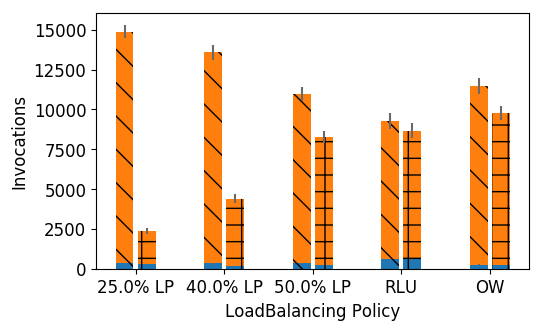
\includegraphics[width=0.4\textwidth]{../Figures/fixed/openload-throughputs.png}
  \caption[fixed-tput]{Throughput with fixed cluster size. Diagonal=High Prio.}
  \label{fig:fixed-tput}
\end{figure}


\paragraph{Deflatable cluster.}
%The low-priority pool is shrunk and the unused servers are removed from the cluster, thus we can reduce the total cluster size.

Service differentiation also allows us to shrink or deflate the \emph{entire cluster.} In this set of experiments, we keep the size of the high priority pool \textbf{fixed}, and shrink the low-priority pool. The free servers are removed from the cluster. 

Figure~\ref{fig:deflat-lat} shows the latency in such a setup.
We are able to shrink the cluster by 25\%, while ensuring the high priority functions are not affected.
Latency improves slightly when the cluster is shrunk slightly (40\% LP) because our fewer servers can still get a low cold-start ratio.
At high levels of cluster shrinkage (25\% LP), latency returns to levels equal to that of the fixed cluster size.
The significant reduction in resources forces low-priority workers to over-commit their resources.
Insufficient memory leads to thrashing of containers being kept warm, and possibly even queueing on occasions when no memory is available.
CPU resources are also forces to be time-shared across running functions.
%, and the low-priority functions are \emph{also not affected} compared to a single cluster (the ``RLU'' case). This is again because of the lower cold-starts we see because of having a smaller cluster partition.
%When the 

%\textbf{Why are the latencies different for the low-priority functions vs. the fixed cluster case?}

\begin{figure}
  \centering 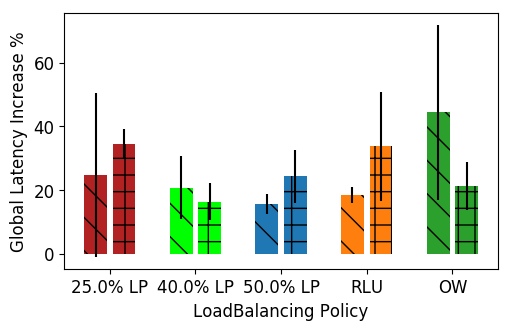
\includegraphics[width=0.4\textwidth]{../Figures/deflat/openload-latencies-cntnorm.png}
  \caption{Latencies with deflatable cluster. Diag=High Prio}
  \label{fig:deflat-lat}
\end{figure}


\begin{figure}
  \centering
  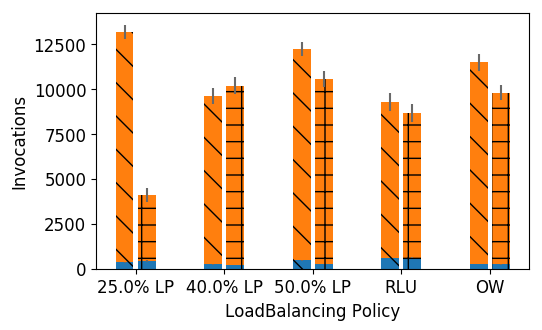
\includegraphics[width=0.4\textwidth]{../Figures/deflat/openload-throughputs.png}
  \caption[fixed-tput]{Throughput with deflatable cluster. Diagonal=High Prio.}
  \label{fig:fixed-tput}
\end{figure}


\paragraph{Impact on individual function latencies.}

The cluster partitioning can have a significant impact on the individual function latencies.
Figure~\ref{fig:violin-0.25} shows the normalized latency distribution of each function, when the cluster is partitioned in a 2:1 split.
We see that the low-priority functions have a higher normalized latency (note the log-scale). 

\begin{figure}
  \centering  \includegraphics[width=0.4\textwidth]{../Figures/timeseries/QoSAwareBalancing-0.25/2-norm_run.png}
  \caption{Latencies of functions under a 2:1 split. Red=high prio. Latencies are normalized to the minimum running time. Low priority functions have higher latencies.}
  \label{fig:violin-0.25}
\end{figure}



\paragraph{Time evolution.}

We now show how the latencies and our objective function changes over time.
We first look at the baseline numbers when both the cluster partitions are the same size, in Figure~\ref{fig:ts-0.5}.
Since both the high and low priority workloads are homogenoeus and have the same resources, we see that the average normalized latencies are also similar.
This indicates that we can use our simple hill-climbing approach, since the ``set point'' can be achieved. 


Next, we look at how the latencies and objective function behaves in a 2:1 cluster split, as seen in Figure~\ref{fig:ts-0.25}. 

\begin{figure}
  \centering  \includegraphics[width=0.4\textwidth]{../Figures/timeseries/QoSAwareBalancing-0.5/4-120.png}
  \caption{Time evolution of the normalized latencies with an evenly partitioned cluster. The avg. normalized latencies for both the pools are pretty close. }
  \label{fig:ts-0.5}
\end{figure}


\begin{figure}
  \centering  \includegraphics[width=0.4\textwidth]{../Figures/timeseries/QoSAwareBalancing-0.25/2-120.png}
  \caption{Time evolution of the normalized latencies with an unevenly partitioned cluster in a 2:1 ratio. The normalized latencies for both the pools are very different. }
  \label{fig:ts-0.25}
\end{figure}


\paragraph{TODO: Dynamic workload and partitioning}



%Delaying improves throughput by ___ 
% Improves e2e latency by ___ ← of a single function 
% Other possible metrics: cost (provider), ability to meet deadlines in highly bursty scenarios.


\subsection{Simulation evaluation}

Load-balancer level techniques implemented and can get graphs quickly.
Will let us show numbers for large clusters and multiple configs.
Main issue is the queueing dispatch model. OWhisk has processor sharing, whereas we are restricted to G/G/k. 

\paragraph{Setup.}
Workload is the azure function trace.
Run on a simulator which implements load balancing and keep-alive.


\begin{figure}[t]
  \centering
  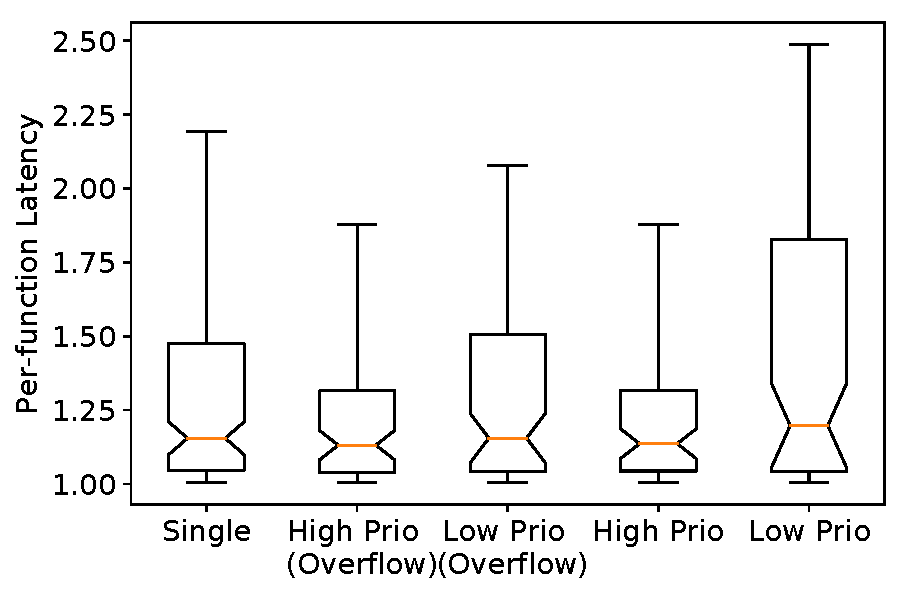
\includegraphics[width=0.4\textwidth]{{../Figures/sim/150-8-1.2-overflow}.pdf}
  \caption{Function latency distribution}
  \label{fig:sim-box-150}
\end{figure}


Figure~\ref{fig:sim-box-150} shows the distribution of per-function latencies across three scenarios.
Compared to the single cluster case: high priority latency is lower.
Low-priority latency is higher.

Currently: there's an anomalous result here: low priority in the overflow case has better latency than in non-overflow scenario.
Note that with overflow, low-priority cluster runs \emph{more} functions, so we should be expecting higher latencies for low-priority functions with overflow.
However: this is occurring due to an accounting error. High priority invocations getting bumped to the low-priority cluster are being accounted as ``low priority''.
This \emph{reduces} the average latency of low-priority, because these bumped functions are bursty, popular, and see a high hit-rate.

This effect can be more starkly observed in Figure~\ref{fig:sim-wlat-150}, which shows the weighted latency, weighted by  the frequency of function invocations. 
Because of the high-priority bursty functions, the low-priority+overflow case has a much lower weighted latency.

%This is currently being fixed (June 3). 


\begin{figure}[t]
  \centering
  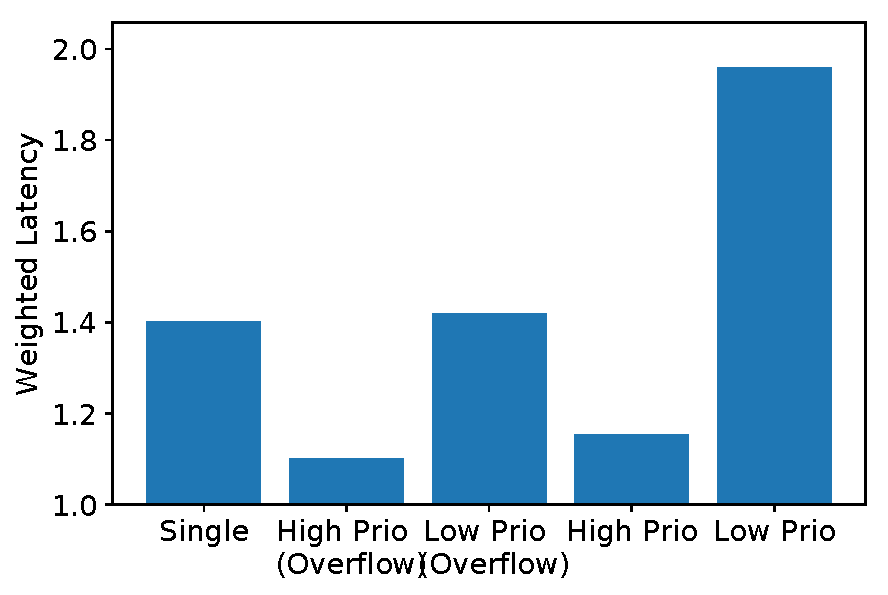
\includegraphics[width=0.4\textwidth]{{../Figures/sim/150-8-1.2-lwlat}.pdf}
  \caption{Overall weighted latency/slowdown.}
  \label{fig:sim-wlat-150}
\end{figure}

Figure~\ref{fig:sim-wlat-150} shows the weighted latency, weighted by  the frequency of function invocations. 



%%% Local Variables:
%%% mode: latex
%%% TeX-master: "paper"
%%% End:
